\documentclass[../Main.tex]{subfiles}
\begin{document}
\chapter{Моменты случайных величин}

\section{Начальный момент}
\[a_k = \mathbb{M}[\xi^k]\] - k-ый начальный момент.

\rmk{Не существует понятие "первый начальный момент". При k = 1 величина называется "математическое ожидание".}
\section{Центральный момент}
\[m_k = \mathbb{M}[(\xi - \mathbb{M}_\xi)^k]\] - k-ый центральный момент.
\rmkb{
\(m_1=0\) всегда.

\(m_2\) называется "дисперсией".
}
\section{Зависимость центральных и начальных моментов}

\(m_3 = \mathbb{M}[(\xi - \mathbb{M}_\xi)^3] = \mathbb{M}[\xi^3 - 3\xi^2\mathbb{M}_\xi + 3\xi(\mathbb{M}_\xi)^2 - (\mathbb{M}_\xi)^3] = \mathbb{M}[\xi^3] - 3\mathbb{M}[\xi^2]\mathbb{M}_\xi+3(\mathbb{M}_\xi)^3 - (\mathbb{M})^ 3 = a_3 - 3a_2a_1 + 2(a_1)^3\)

\rmk{Эти формулы позволяют получить упрощение вычислений. Числа возле начальных моментов можно получить из треугольника Паскаля (см. ниже), где ряд - порядок центрального момента}

\begin{figure}
    \centering
    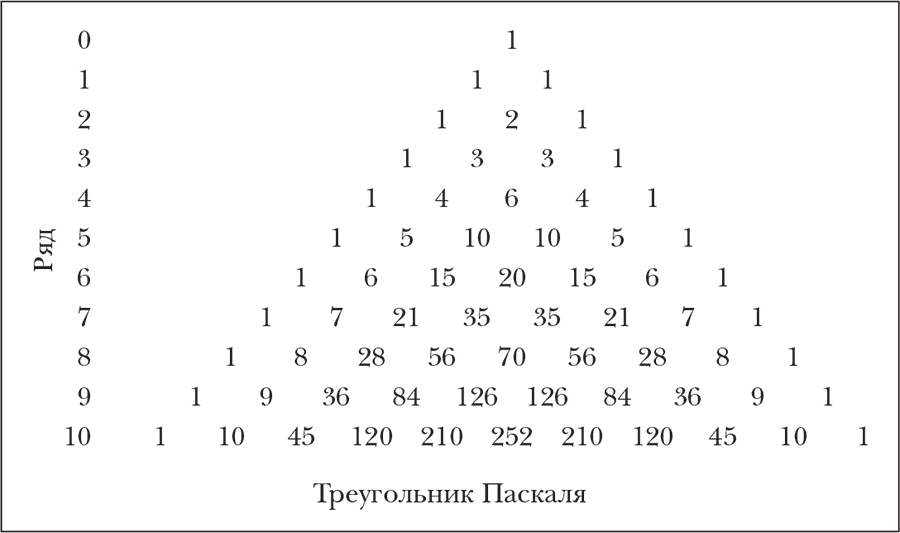
\includegraphics[width=0.9\linewidth]{Images/паскаль.png}
\end{figure}

\section{Абсолютные моменты}
\subsection{Абсолютный начальный момент}

\[\mathbb{M}[|\xi|^k]\] - k-ый абсолютный начальный момент = начальный момент модуля.

\subsection{Абсолютный центральный момент}

\[\mathbb{M}[|\xi - \mathbb{M}_\xi|^k]\] - k-ый абсолютный центральный момент.

\section{Медиана}

Характеристика, важная для дискретных случайных величин.

\defn{Медиана}{
Такое число l, что \(\mathbb{P}(\xi < l) = \mathbb{P}(\xi \geq l)\).

При этом \(\mathbb{F}_\xi(l)=\dfrac{1}{2}\)
}

\rmk{Квантиль — граница деления выборки или совокупности на равные по размеру смежные подгруппы.}

\(x_p\) (квантиль порядка \(p\)) \Rightarrow \(\mathbb{P}(\xi < x_p) = p \leftrightarrow \mathbb{F}_\xi(x_p) = p,\ 0<p<1\).

\(\mathbb{P}(\xi < x_p) = p\). При \(p = \dfrac{1}{2}\ l \ -\) медиана.

\section{Мода}

\rmk{Мода — это точка, в которой плотность (для непрерывных случайных величин) или вероятность (для дискретных случайных величин) достигает своего максимума.}

Для дискретной случайной величины \(x_{i-1}<x_i=m<x_{i+1}, \) если \(\mathbb{P}_i \geq \mathbb{P}_{i-1}\) и \(\mathbb{P}_i \geq \mathbb{P}_{i+1}\), то есть такое значение, что вероятность в этой точке/точках не меньше вероятности в соседних точках.

Для непрерывной случайной величины мода - точка локального максимума плотности.

\defn{Распределения}{
\begin{itemize}
    \item 1 точка моды - унимодулярное распределение;
    \item 2 точки моды - бимодулярное распределение;
    \item 3+ точки моды - полимодулярное распределение.
\end{itemize}
}

\section{Только у непрерывных случайных величин}

\subsection{Коэффициент асимметрии}

\rmk{Коэффициент асимметрии описывает, насколько распределение случайной величины \(\xi\) асимметрично относительно своего среднего значения (или центра). Он показывает, есть ли "перекос" влево или вправо.}

\defn{Коэффициент асимметрии}{
\(\beta = \dfrac{M[(ξ−μ)^3]}{σ^3}\), где числитель - третий центральный момент, а знаменатель - среднее квадратическое отклонение в кубе.
}

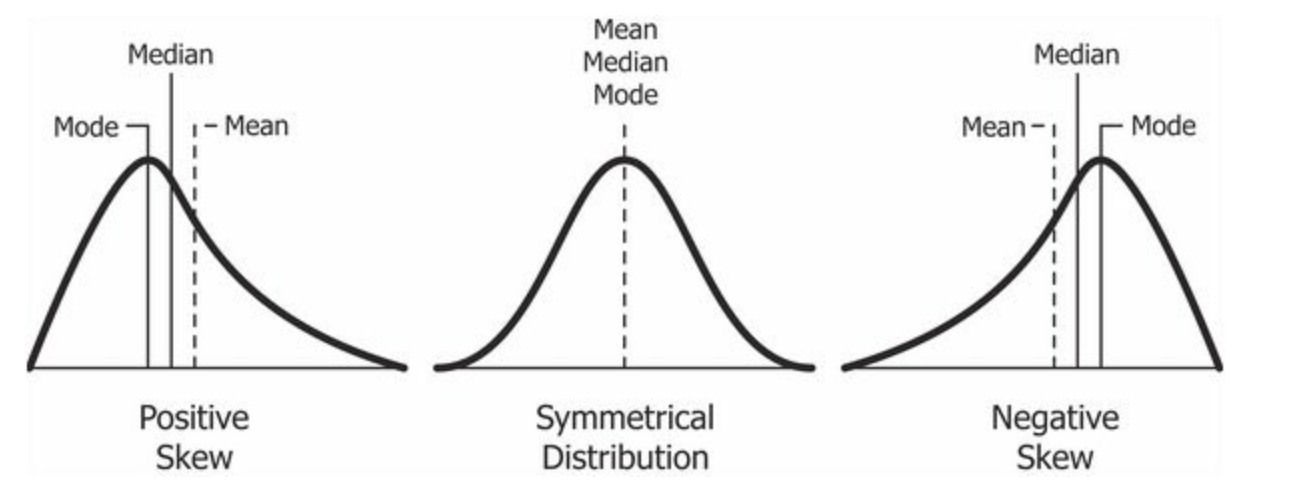
\includegraphics[width=\linewidth]{Images/распределение.png}
\begin{enumerate}
    \item \(\beta = 0 \Rightarrow\) распределение симметрично (например, нормальное распределение).
    \item \(\beta > 0 \Rightarrow\) положительная асимметрия (правый хвост длиннее или тяжелее).
    \item \(\beta < 0 \Rightarrow\) отрицательная асимметрия (левый хвост длиннее или тяжелее).
\end{enumerate}

\subsection{Коэффициент эксцесса}

\rmk{Коэффициент эксцесса описывает "остроту" пика распределения и "тяжесть" его хвостов по сравнению с нормальным распределением. Он показывает, насколько распределение "вытянуто" или "сплющено".}

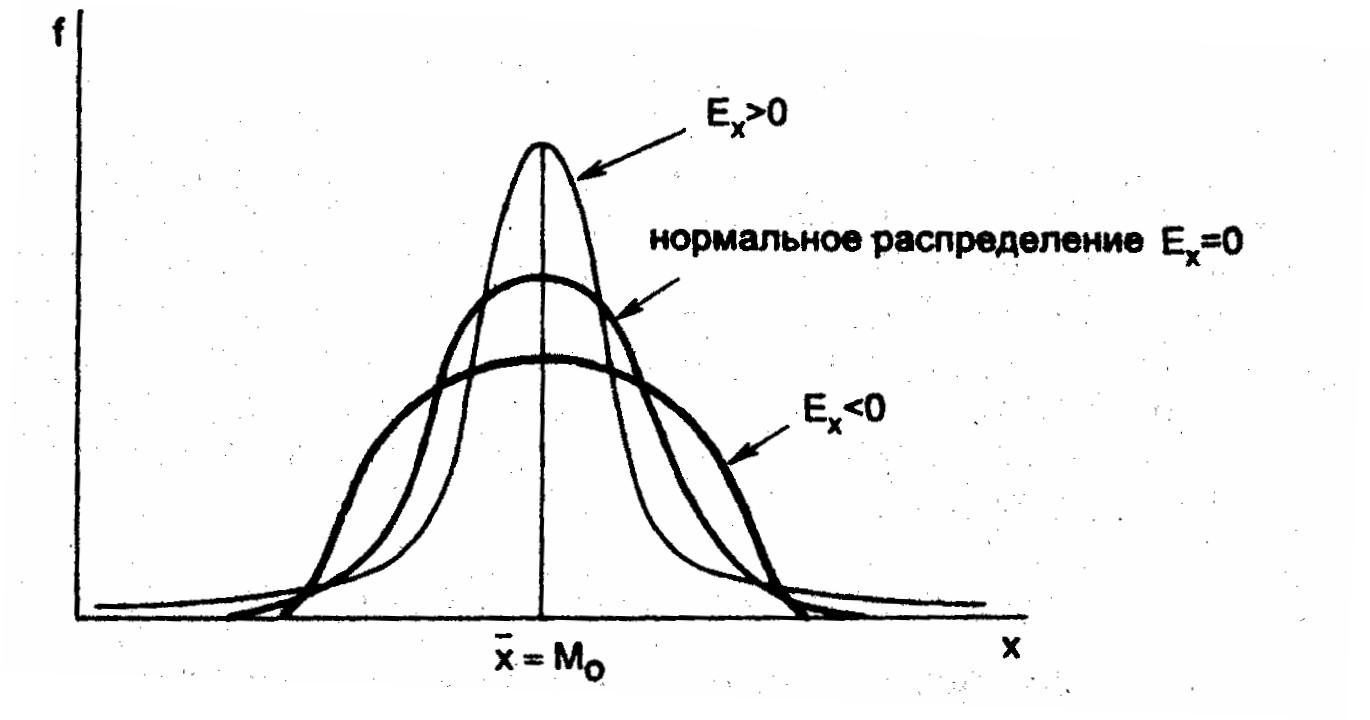
\includegraphics[width=0.8\linewidth]{Images/эксцесс.jpg}

\defn{Коэффициент эксцесса}{
\(\gamma = \dfrac{M[(ξ−μ)^3]}{σ^3} - 3\), где числитель - третий центральный момент, а знаменатель - среднее квадратическое отклонение в кубе, а вычитание 3 делается, чтобы сравнивать с нормальным распределением, у которого \(\beta = 0\).
}

\fact{В симметричном унимодулярном распределении (например, нормальном) мода, медиана и матожидание совпадают.
В асимметричном распределении они расходятся. Например, при положительной асимметрии: мода < медиана < матожидание.}

\section{Только у дискретных случайных величин}

\subsection{Многоугольник распределения}

\defn{Многоугольник распределения}{
Ломаная линия, отрезки которой последовательно соединяют точки с координатами (\(x_i, \mathbb{P}_i\)), где \(x_i\) — возможные значения случайной величины, а \(\mathbb{P}_i\) — соответствующие вероятности.
}

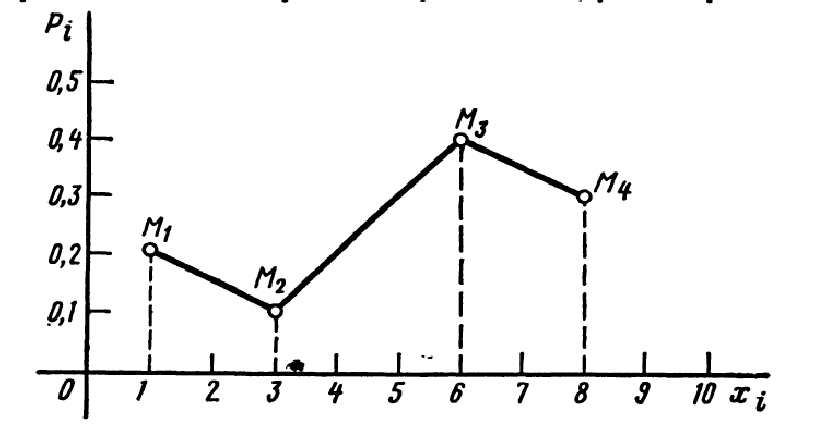
\includegraphics[width=0.8\linewidth]{Images/многоугольник.png}

Он строится в прямоугольной системе координат, в которой по оси абсцисс отсчитываются значения случайной величины, а по оси ординат — их вероятности. 3

\end{document}